%%%%%%%%% ANALYSIS
\section{Analysis}
\label{sec:05_analysis}

\subsection{Visualization of Perturbations}
\begin{figure}
    \centering
    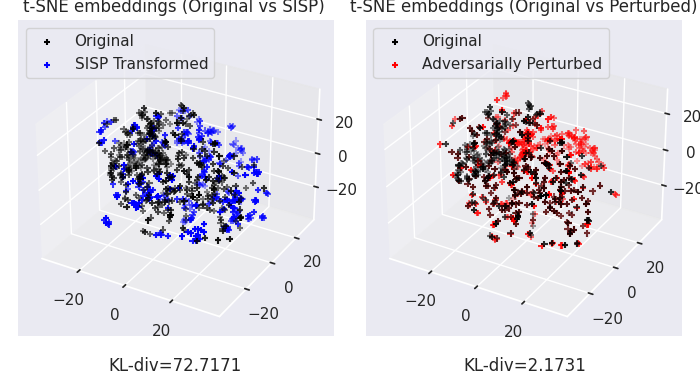
\includegraphics[width=\linewidth]{sdro/images/tsne_orig_both_pplx_5.png}
    \caption{
    Comparison of original sentences (black) with \textit{(left)} SISP-transformed sentences (blue) and \textit{(right)} \straightepsilon-bounded perturbations
    as a tSNE plot.
    }
    \label{fig:tsne}
\end{figure}
In order to quantify the diverse and larger semantic transformations compared to additive perturbations, 
we study the tSNE~\citep{van2008visualizing} embeddings of (i) original samples from NLVR$^2$ ($P$), (ii) their SISP-transformed versions ($P_{SISP}$), and (iii) their adversarially perturbed versions ($P_{adv}$).
Input sentences are encoded using the UNITER text encoder for (i) and (ii), and the adversarial perturbation mechanism~\citep{gan2020large} for (iii).
3D tSNE embeddings are visualized in Figure~\ref{fig:tsne}; SISP transformed sentences (blue) are farther away than the perturbed versions.
This shift is quantified by the KL-divergence~\citep{kullback1951information} between the distributions, with $D_{KL}(P_{SISP}||P) > D_{KL}(P_{adv}||P)$ implying that the diversity of SISP transformations is higher.


\subsection{Comparison of Model Calibration}
\begin{figure}
    \centering
    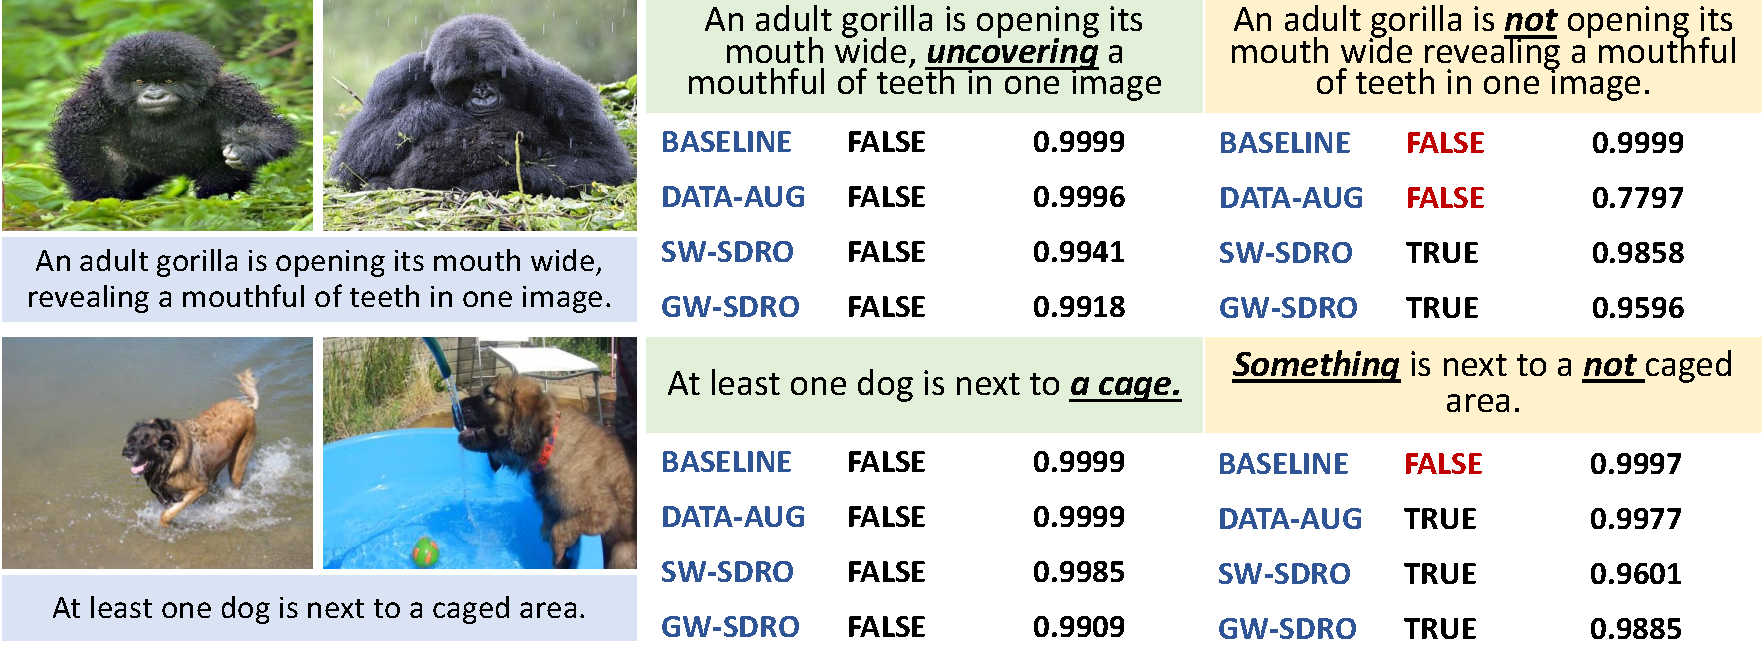
\includegraphics[width=\linewidth]{sdro/images/predictions_qualitative_2.pdf}
    \caption{
    Original test inputs for NLVR$^2$ with their respective SP (green) and SI (yellow) test samples and the prediction and confidence of models with VILLA backbone.
    Wrong predictions are highlighted in red.
    }
    \label{fig:qualitative}
\end{figure}
Figure~\ref{fig:qualitative} contains qualitative examples from NLVR$^2$ to compare output probabilities.
We observe that SDRO models have higher clean accuracy, but lower confidence in the predictions than baseline and \textit{data-aug} methods.
\paragraph{Reliability Diagrams.}
\begin{figure}
    \centering
    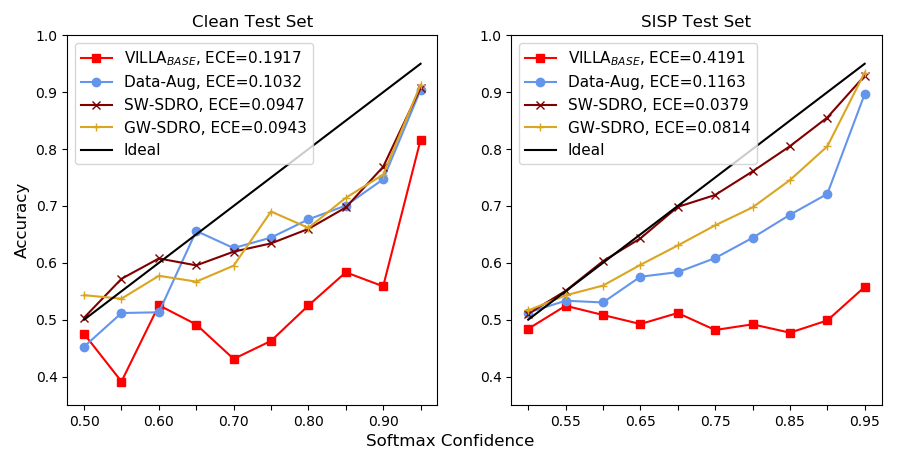
\includegraphics[width=\linewidth]{sdro/images/reliability.png}
    \caption{Comparison of reliability curves on the clean test set \textit{(left)} and SISP test set \textit{(right)}.}
    \label{fig:reliability}
\end{figure}
To validate this observation at scale, we use reliability diagrams to visualize model calibration~\citep{niculescu2005predicting}, and plot model accuracy as a function of confidence.
We use the softmax probability $\hat{p}$ of the predicted class as model confidence, split the range of probabilities into $M=20$ equal-sized bins, and calculate bin accuracy $acc(B_m)$ and bin confidence $conf(B_m)$~\citep{guo2017calibration}.
If $B_m$ is the set of all samples that fall in the $m^{th}$ bin,
\begin{align}
    acc(B_m) &\triangleq \frac{1}{|B_m|}\sum_{X_i\in B_m}\mathbbm{1}(\hat{y}_i = y_i), \\
    conf(B_m) &\triangleq \frac{1}{|B_m|}\sum_{X_i\in B_m} \hat{p}_i .
\end{align}
A model with perfect calibration should have a reliability diagram such that $$acc(B_m)=conf(B_m)$$.
We also report Expected Calibration Error~\citep{naeini2015obtaining} over all $n$ test samples:
\begin{equation}
    ECE=\sum_{m=1}^M\frac{|B_m|}{n}|acc(B_m){-}conf(B_m)|.
\end{equation}


Reliability diagrams and corresponding ECE values for the baseline VILLA trained with naive data augmentation and SDRO methods for NLVR$^2$ are shown in Figure~\ref{fig:reliability}.
On both the clean test set and SISP test set, SDRO models have the lowest ECE.
While the ECE for SDRO is marginally better than data augmentation for the clean test set, SDRO is much better calibrated for the SISP test set, with SW-SDRO closest to ideal calibration.

\subsection{Size of Training Dataset}
We evaluate models trained on small subsets of the original dataset, and compare their performance in Figure~\ref{fig:lowres}.
SDRO models are significantly better at all sizes of training datasets as shown by accuracy and AUC (area under the curve).
Notably, SDRO models trained with only $10\%$ ($\sim8.6K$) samples have performances similar to the baseline trained with $30\%$ samples;
SDRO models with $20\%$ data are better than the baseline model with $40\%$ data.
While models trained with naive augmentation saturate below SOTA, at ${\sim}80\%$ data size, SDRO models cross the existing SOTA of $78.39\%$.

\begin{figure}[t]
    \centering
    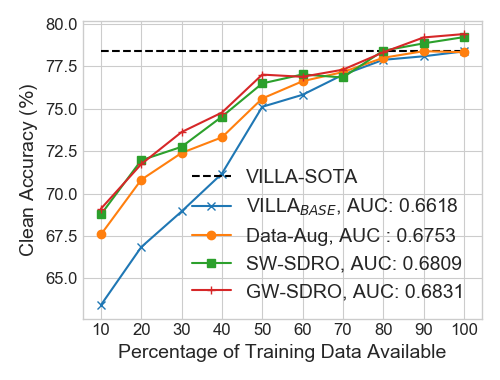
\includegraphics[width=0.49\linewidth]{sdro/images/lowResource_auc.png}
    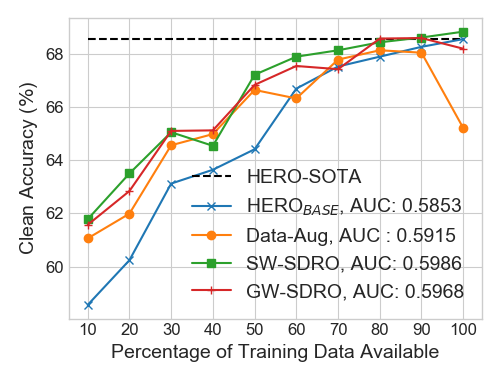
\includegraphics[width=0.49\linewidth]{sdro/images/violin_lowResource_auc.png}
    \caption{
    Effect of size of training data \textit{(left)} NLVR$^2$, \textit{(right)} VIOLIN.
    SDRO models are consistently better than baselines, even in low-data settings. 
    }
    \label{fig:lowres}
\end{figure}

\subsection{Ablation Studies}
\begin{figure}[t]
    \centering
    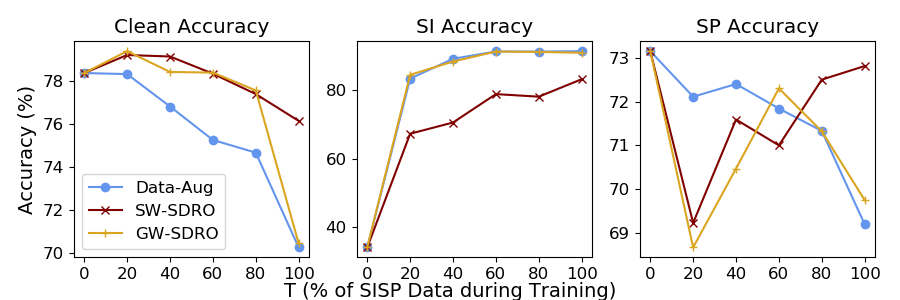
\includegraphics[width=\linewidth]{sdro/images/T_as_curve.png}
    \caption{
    Plots showing the effect of the percentage of augmented samples on Clean, SP, and SI accuracies on NLVR$^2$, when using data-augmentation, and SDRO.
    }
    \label{fig:NLVR2_ablation_T}
\end{figure}
\paragraph{Proportion of Augmented Samples.}
The final dataset has the same size as the original training set, but with T$\%$ transformed samples and $(100{-}T)\%$ original samples.
The effect of this hyperparameter $T$ is reported in Figure~\ref{fig:NLVR2_ablation_T} as a percentage improvement of accuracy w.r.t.\ VILLA$_{BASE}$.
An {optimal value of $T{=}20\%$ leads to improvements in clean accuracy}, but a larger proportion of augmented samples degrades performance.
Similarly, higher $T$ leads to higher robust accuracy, pointing to a \textul{trade-off between clean accuracy and robust accuracy at values of $T$ higher than the optimal}.
This conforms with similar findings from~\citet{tsipras2019robustness}.
While models trained with naive data-augmentation have better SISP accuracy than SDRO models as in Table~\ref{tab:results_nlvr2}, they do so by sacrificing clean accuracy, while SDRO models improve along both dimensions compared to the baselines.

\paragraph{Contributions of SI and SP independently:}
\begin{table}
    \centering
    \resizebox{\linewidth}{!}{
    \begin{tabular}{@{}l ccc c ccc c ccc@{}}
        \toprule
        \multirow{2}{*}{\textbf{Model}} & \multicolumn{3}{c}{SP only} & \hphantom & \multicolumn{3}{c}{SI Only} & \hphantom & \multicolumn{3}{c}{Both} \\ 
         \cmidrule{2-4} \cmidrule{6-8}  \cmidrule{10-12}
         & Clean & SP & SI && Clean & SP & SI && Clean & SP & SI \\
        \midrule
        Data-Aug & 76.07 & 74.89 & 35.77 && 69.51 & 53.68 & 94.89 && 78.34 & 72.11 & 84.44 \\
        SW-SDRO & 79.79 & 76.93 & 30.72 && 79.27 & 55.53 & 88.76 && 79.23 & 69.23 & 67.35 \\
        GW-SDRO & 79.46 & 75.72 & 33.04 && 79.13 & 54.31 & 93.25 && 79.41 & 68.67 & 84.54 \\
        \bottomrule
    \end{tabular}
    }
    \caption{Comparison of performance when only SP, only SI, or both types of transformations are performed.}
    \label{tab:analysis_si_sp_all}
\end{table} 
We analyze which of the two categories (semantics-inverting (SI) or semantics-preserving (SP)) is the most effective by performing SDRO with only SI transforms, or with only SP transforms, and when using both.
Table~\ref{tab:analysis_si_sp_all} shows that SDRO models trained only with SI suffer in terms of SP robustness and vice versa.
However, there is still an increase in clean accuracy in both cases.
This indicates that \textul{both SI and SP contribute towards improvements in robustness and clean accuracy.}


\paragraph{Transformations of only \texttt{True} statements:}
\begin{table}
    \centering
    % \footnotesize
    % \resizebox{\linewidth}{!}{
    \begin{tabular}{@{}l ccc c ccc@{}}
        \toprule
        \multirow{2}{*}{\textbf{Model}} & \multicolumn{3}{c}{SISP~(Pos)} & \hphantom & \multicolumn{3}{c}{SISP~(All)} \\ 
         \cmidrule{2-4} \cmidrule{6-8}
         & Clean & SP & SI && Clean & SP & SI \\
        \midrule
        Data-Aug & 78.23 & 68.02 & 57.48 && 78.34 & 72.11 & 84.44 \\
        SW-SDRO  & 78.81 & 62.06 & 66.07 && 79.23 & 69.23 & 67.35 \\
        GW-SDRO  & 79.10 & 63.47 & 62.29 && 79.41 & 68.67 & 84.54\\
        \bottomrule
    \end{tabular}
    % }
    \caption{Comparison of performance if only positive samples 
    % or both positive or negative samples 
    % i.e.\ samples with \texttt{True} labels 
    are used as inputs for SISP transformations
    % ,  transformations over both positive and negative samples.
    }
    \label{tab:analysis_pos_all}
\end{table} 
Transforming \textit{False} (negative) statements can lead to ambiguous and subjective meanings~\citep{russell1905denoting}.
We investigate if transforming only \textit{True} (positive) statements is better than transforming both \textit{True} and \textit{False} statements.
Table~\ref{tab:analysis_pos_all} shows that SISP transformations of both types of statements lead to higher clean accuracy and robustness.

\subsection{Robustness to Text-Attacks}

% \begin{table}[t]
%     \centering
%     \resizebox{\linewidth}{!}{
%     \begin{tabular}{@{}cl ccccccc@{}}
%         \toprule
%         % \multirow{2}{*}{\textbf{Model}} & \multicolumn{7}{c}{\textbf{Text Attack Categories}} \\
%         % \textbf{Dataset}
%         & \textbf{Model} & \textbf{CR} & \textbf{CS} & \textbf{CL} & \textbf{EDA} & \textbf{Emb} & \textbf{WN} & \textbf{Avg.}\\
%         \midrule
%         % LX          & 74.38 & 72.45 & 70.72 & 67.73 & 71.26 & 72.12 & 71.44 \\
%         % LX + SDRO   & 70.18 & 67.96 & 65.94 & 64.29 & 69.05 & 66.49 & 67.32 \\
%         % \midrule  
%         % UN          & 75.35 & 75.44 & 73.99 & 69.02 & 74.96 & 73.45 & 73.70 \\
%         % UN + SDRO   & 75.71 & 75.35 & 71.14 & 68.84 & \underline{76.44} & 75.24 & 73.79 \\
%         % \midrule 
%         \multirow{2}{*}{NLVR$^2$} 
%         & VILLA          & 77.45 & 74.38 & \underline{74.42} & 69.62 & 75.45 & 75.87 & 74.52 \\
%         & \quad + SDRO   & \underline{78.51} & \underline{77.20} & 72.06 & \underline{71.08} & 75.77 & \underline{76.41} & \textbf{75.17}\\
%         \midrule
%         \multirow{2}{*}{VIOLIN} 
%         & HERO          & 66.08  & 63.00 & 68.58 & 60.89 & 63.81 & 63.38 & 64.29 \\
%         & \quad + SDRO   & 68.70 & 64.95 & 68.96 & 61.32 & 65.54 & 64.61 & 65.68 \\
%         \midrule
%         \multirow{2}{*}{\shortstack{VQA \\Yes/No}} 
%         & VILLA          & 80.49 & 75.74 & 84.87 & 74.64 & 78.63 & 76.39 & 78.45 \\
%         & \quad + SDRO   & 85.99 & 84.52 & 84.10 & 87.02 & 84.25 & 84.03 & 84.99 \\
%         \bottomrule
%     \end{tabular}
%     }
%     \caption{Performance on ``text-attack''~\cite{morris2020textattack} versions of the NLVR$^2$, VIOLIN, and VQA-Yes/No test sets. CR: CLARE; CS: CharSwap, CL: Check-List, EDA: Easy Data Augmentation, Emb: Embedding-based, WN: WordNet-based.}
%     \label{tab:text_attack}
% \end{table}

\begin{table}
    \centering
    % \small
    % \resizebox{\linewidth}{!}{
    \begin{tabular}{@{}cl ccccccc@{}}
        \toprule
        & \textbf{Model} & \textbf{CR} & \textbf{CS} & \textbf{CL} & \textbf{EDA} & \textbf{Emb} & \textbf{WN} & \textbf{Avg.}\\
        \midrule
        \multirow{2}{*}{NLVR$^2$} 
        & VILLA          & 77.5 & 74.4 & \underline{74.4} & 69.6 & 75.5 & 75.9 & 74.5 \\
        & \quad + SDRO   & \underline{78.5} & \underline{77.2} & 72.1 & \underline{71.1} & 75.8 & \underline{76.4} & \textbf{75.2}\\
        \midrule
        \multirow{2}{*}{VIOLIN} 
        & HERO          & 66.1  & 63.0 & 68.6 & 60.9 & 63.8 & 63.4 & 64.3 \\
        & \quad + SDRO   & 68.7 & 65.0 & 69.0 & 61.3 & 65.5 & 64.6 & 65.7 \\
        \midrule
        \multirow{2}{*}{\shortstack{VQA \\Yes/No}} 
        & VILLA          & 80.5 & 75.7 & 84.9 & 74.6 & 78.6 & 76.4 & 78.5 \\
        & \quad + SDRO   & 86.0 & 84.5 & 84.1 & 87.0 & 84.3 & 84.0 & 85.00 \\
        \bottomrule
    \end{tabular}
    % }
    \caption{Performance on ``text-attack'' of NLI test set.
    % ~\cite{morris2020textattack} versions of the NLVR$^2$, VIOLIN, and VQA-Yes/No test sets. 
    % CR: CLARE, CS: CharSwap, CL: Check-List, EDA: Easy Data Aug, Emb: Embedding-based, WN: WordNet-based.
    }
    \label{tab:text_attack}
\end{table}
We utilize automated adversarial attack recipes~\citep{morris2020textattack}:
CLARE (CR)~\citep{li2021contextualized}, character-swap (CS)~\citep{pruthi2019combating}, Checklist (CL)~\citep{ribeiro2020beyond}, EDA~\citep{wei2019eda}, counter-fitted embeddings (Emb)~\citep{alzantot2018generating}, and WordNet-based swap~\citep{ren2019generating}.
Table~\ref{tab:text_attack} shows results using the best backbone and our SDRO model.
On NLVR$^2$, VILLA+SDRO is better than VILLA for 4 out of 6 attack categories, and $0.65\%$ on average.
On VIOLIN, HERO+SDRO outperforms the baseline on all attack categories, leading to an average gain of $1.39\%$.
On VQA-Yes/No, VILLA+SDRO outperforms the baseline on all attack categories, and $6.54\%$ on average.

